\documentclass[12pt,fleqn]{article}\usepackage{../common}
\begin{document}
Paralel Lojistik Regresyon, Esle/Indirge

Lojistik regresyon kodunu esle-indirge (map-reduce) uzerinden paralelize
etmek icin literature [1-7] bakinca, genel yaklasimin makinalara bolunen
veri parcalari uzerinde ayri ayri graydan cikisinin (gradient ascent)
isletilmesi ve sonuc $\theta$'larin son bir makinada ortalamasinin alinmasi
oldugunu goruruz.

Daha onceki lojistik regresyon yazimizda iki farkli gradyan cikis
algoritmasi gormustuk. Bu algoritmalardan kullanacagimiz daha basit olani,
her dongude alpha'yi degistiren versiyon degil tek alpha kullanan, ve kod
icinde zar atan degil, veriyi sirayla isleyen. Bunun birkac sebebi var,
oncelikle altta gorecegimiz uzere veriyi Hadoop'a vermeden once kendimiz
karistiracagiz, yani kod icinde zar atmaya gerek kalmayacak. Ikincisi pek
cok makinada islem yapildigi icin tek bir sabit uzerinden azaltma yapmak
mumkun degil (fakat her isleyicinin -degismeyen- kendine has / ayri bir
sabiti olabilir, bu konuyu ileride isleyebiliriz), bu sebeple ve basitlik
amaciyla tek sabitli kod kullanildi. Ayrica artik dongu (iterasyon) yok,
yani veri bastan sona bir kez tarandi mi, o makinanin islemi bitecek. Fakat
buyuk veri ortaminda (ki zaten onun icin Hadoop kullaniyoruz herhalde)
elimizde o kadar cok veri olacak ki bu verinin tamamini isleyince zaten
100,200 kere donguyu isletmek ile ayni etkiyi almis oluyoruz.

Ornek veri olarak alttakini urettik,

\begin{lstlisting}[language=Python]
from pandas import *
mean1 = [10,10]
mean2 = [20,20]
cov = [[5,0],[0,5]]
d1 = DataFrame(np.random.multivariate_normal(mean1,cov,10000))
d2 = DataFrame(np.random.multivariate_normal(mean2,cov,10000))
d1['labels'] = 1
d2['labels'] = 0
data = DataFrame(np.vstack((d1,d2)))
data.to_csv("testSet.txt",sep='\t',index=None,header=None)
print data[:4]
\end{lstlisting}

\begin{verbatim}
           0          1  2
0  12.240490  13.455531  1
1  13.866198   6.745407  1
2   8.483480  11.583482  1
3  11.693351  10.414605  1
\end{verbatim}

\begin{lstlisting}[language=Python]
%pylab inline
plt.plot(d1.ix[:,0],d1.ix[:,1],'b.')
plt.hold(True)
plt.plot(d2.ix[:,0],d2.ix[:,1],'r.')
plt.hold(True)
plt.savefig('logreg1.png')
\end{lstlisting}

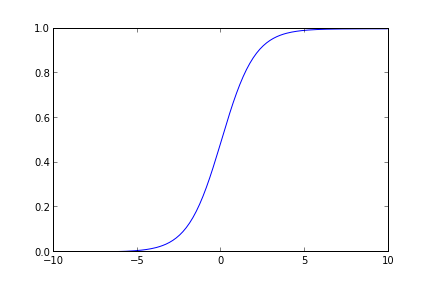
\includegraphics[height=4cm]{logreg1.png}













\end{document}
